\documentclass[10pt, xcolor=dvipsnames]{beamer}

% There are many different themes available for Beamer. A comprehensive
% list with examples is given here:
% http://deic.uab.es/~iblanes/beamer_gallery/index_by_theme.html
% You can uncomment the themes below if you would like to use a different
% one:
%\usetheme{AnnArbor}
%\usetheme{Antibes}
%\usetheme{Bergen}
%\usetheme{Berkeley}
%\usetheme{Berlin}
%\usetheme{Boadilla}
%\usetheme{boxes}
%\usetheme{CambridgeUS}
%\usetheme{Copenhagen}
%\usetheme{Darmstadt}
%\usetheme{default}
%\usetheme{Frankfurt}
%\usetheme{Goettingen}
%\usetheme{Hannover}
%\usetheme{Ilmenau}
%\usetheme{JuanLesPins}
%\usetheme{Luebeck}
%\usetheme{Frankfurt}
\usetheme{Madrid}
%\usetheme{Malmoe}
%\usetheme{Marburg}
%\usetheme{Montpellier}
%\usetheme{PaloAlto}
%\usetheme{Pittsburgh}
%\usetheme{Rochester}
%\usetheme{Singapore}
%\usetheme{Szeged}
%\usetheme{Warsaw}

\usepackage[utf8]{inputenc}
\usepackage[english]{babel}
\usepackage{ragged2e}
\usepackage{bbding}
%\usepackage{enumitem}
\usepackage{mathtools}
\usepackage{indentfirst}
\usepackage{graphicx}
\usepackage{float}
\usepackage{hyperref}
\usepackage{mathtools}
\usepackage{preview}
\usepackage{xcolor}
\usepackage{color}
\usepackage{listings}
\usepackage{float}
\usepackage[caption = false]{subfig}
\usepackage{pdfpages}
\usepackage{multirow}
\usepackage{array}
\usepackage{makecell}
\usepackage{bm}
\usepackage{caption}
\usepackage{cancel}
\usepackage{anyfontsize}
\usepackage{etoolbox}
\usepackage{amsmath}
\usepackage{amssymb}
\usepackage{mathtools}
\usepackage{natbib}
\usepackage[flushleft]{threeparttable}
\usepackage{booktabs}
\usepackage{caption}
\usepackage{adjustbox}
\usepackage{appendixnumberbeamer}
\usepackage{pifont}
\usepackage{amsmath}
\usepackage{amssymb}
\usepackage{longtable}
\usepackage[percent]{overpic}



\setbeamercolor{titlelike}{parent=structure}
\definecolor{UBCblue}{rgb}{0.04706, 0.13725, 0.32}
\colorlet{UBCblue2}{UBCblue!70!white}
\usecolortheme[named=UBCblue]{structure}

\makeatletter
\setbeamertemplate{footline}
{
  \leavevmode%
  \hbox{%
  \begin{beamercolorbox}[wd=.4\paperwidth,ht=2.25ex,dp=1ex,center]{author in head/foot}%
    \usebeamerfont{author in head/foot} \insertshortauthor %\hspace*{1em}(\insertshortinstitute)
  \end{beamercolorbox}%
  \begin{beamercolorbox}[wd=.5\paperwidth,ht=2.25ex,dp=1ex,center]{title in head/foot}%
    \usebeamerfont{title in head/foot} \insertshorttitle
  \end{beamercolorbox}%
  \begin{beamercolorbox}[wd=.1\paperwidth,ht=2.25ex,dp=1ex,center]{date in head/foot}%
    \usebeamerfont{date in head/foot}
    \insertframenumber{} / \inserttotalframenumber\hspace*{2ex} 
  \end{beamercolorbox}}%
  \vskip0pt%
}
\makeatother

\renewcommand{\arraystretch}{1.2}
\renewcommand{\raggedright}{\leftskip=0pt \rightskip=0pt plus 0cm}
\newcolumntype{C}[1]{>{\centering\let\newline\\\arraybackslash\hspace{0pt}}m{#1}}

\hypersetup{
    colorlinks=true,
    linkcolor=UBCblue,
    citecolor=UBCblue,
    filecolor=magenta,      
    urlcolor=blue,
    allcolors=.
}
\setbeamercolor{button}{bg=UBCblue2,fg=white}
\newcommand\fnote[1]{\captionsetup{font=tiny}\caption*{#1}}
\newcommand\fnotev[1]{\captionsetup{font=scriptsize}\caption*{#1}}
\setbeamertemplate{caption}[numbered]


%\justifying
\urlstyle{same}
%\usefonttheme{serif}

%------------------------
%------------------------

\date{}

%------------------------
%------------------------
%----------------------------------------------------------------------------------------
%	TITLE PAGE
%----------------------------------------------------------------------------------------------------------------
%------------------------

\title[Landlord Responses to Changes in Tenant Protections]{Are Slumlords Necessary: \\Landlord Responses to Changes in Tenant Protections} % The short title appears at the bottom of every slide, the full title is only on the title page
\author[Joe Fish]{Joe Fish}


\begin{document}

\begin{frame}
\titlepage % Print the title page as the first slide
\end{frame}


\begin{frame}{Recap of Project}
   \textbf{ What does a city do about slumlords?}
   \begin{itemize}
    \item Most US cities have awful tenant protections
    \item Tenants perceived as risky face large barriers to finding housing. Lots of rental listings will have "no eviction, no conviction" clauses, effectively locking them out of large parts of the rental market. This is true for private and public landlords.
    \item Landlords that rent to risky tenants are providing a service, these landlords are also much more likely to be predatory.
    \item When advocacy groups push for stronger tenant protections, landlords (public and private) argue that increased tenant protections would make them unable to be effective landlords. Thus, it's ex ante, unclear what the best way to regulate low income landlords is.
\end{itemize}
\end{frame}

\begin{frame}{Recap of Stylized Facts}
    High Filing Units charge more, conditional on a bunch of observables
    \tiny
    \begingroup
\centering
\begin{tabular}{lc}
   \tabularnewline \midrule \midrule
   Dependent Variable:     & Log Median Rent\\  
   Model:                  & (1)\\  
   \midrule
   \emph{Variables}\\
   Filing Rate: 10-20\%    & 0.0087\\   
                           & (0.0069)\\   
   Filing Rate: 20-30\%    & 0.0303$^{***}$\\   
                           & (0.0084)\\   
   Filing Rate: 30\%+      & 0.0277$^{**}$\\   
                           & (0.0108)\\   
   \midrule
   \emph{Fixed-effects}\\
   Census Block Group-year & Yes\\  
   Decade Built            & Yes\\  
   Number of Stories       & Yes\\  
   Data Source             & Yes\\  
   Quality Grade           & Yes\\  
   Exterior Condition      & Yes\\  
   Building Type           & Yes\\  
   \midrule
   \emph{Fit statistics}\\
   Observations            & 131,719\\  
   \midrule \midrule
   \multicolumn{2}{l}{\emph{Clustered (parcel) standard-errors in parentheses}}\\
   \multicolumn{2}{l}{\emph{Signif. Codes: ***: 0.01, **: 0.05, *: 0.1}}\\
\end{tabular}
\par\endgroup

    
\end{frame}

\begin{frame}{Recap of Model}
    \begin{enumerate}
    \item Each renter chooses a probability distribution over the homes to send out one application. The probability distribution is such that $\pi_t = (\pi_t(1) \dots \pi_t(k))$ with $\sum_{k = 1}^{K} \pi_t(k)=1$
    \item Each renter chooses one home to apply to, drawn from $\pi_t$
    \item For type B landlords, if a unit receives multiple applications, it chooses one, breaking ties randomly
    \item For type A landlords, they first choose randomly between high types and then choose randomly between low types if no high types apply.
    \item unmatched landlords and tenants produce nothing and get zero payoff
    \begin{itemize}
        \item justified because it seems unreasonable to expect landlords and tenants to coordinate application behavior
    \end{itemize}

\end{enumerate}
\end{frame}

\begin{frame}{Issues}
    \begin{itemize}
        \item Stylized facts not super robust
        \item Calibration wasn't working correctly; (matching pennies issue in the code)
        \item Hard to calibrate
    \end{itemize}
    
\end{frame}

\begin{frame}{New Ideas}
    \begin{itemize}
        \item Landlord responses to changes in tenant protections
        \begin{itemize}
            \item A couple papers that try to do this. I think they're missing how the econ works; the relevant margin isn't landlord exit, it's landlords changing how they manuever vacancies
        \end{itemize}
        \item Who sets prices in response to demand shocks; idea is that adjustment is faster in markets with more units / more corporate owned units
    \end{itemize}
    
\end{frame}

\begin{frame}{High Evicting Landlords Increased Prices Post-COVID}
    \begin{figure}
        \centering
        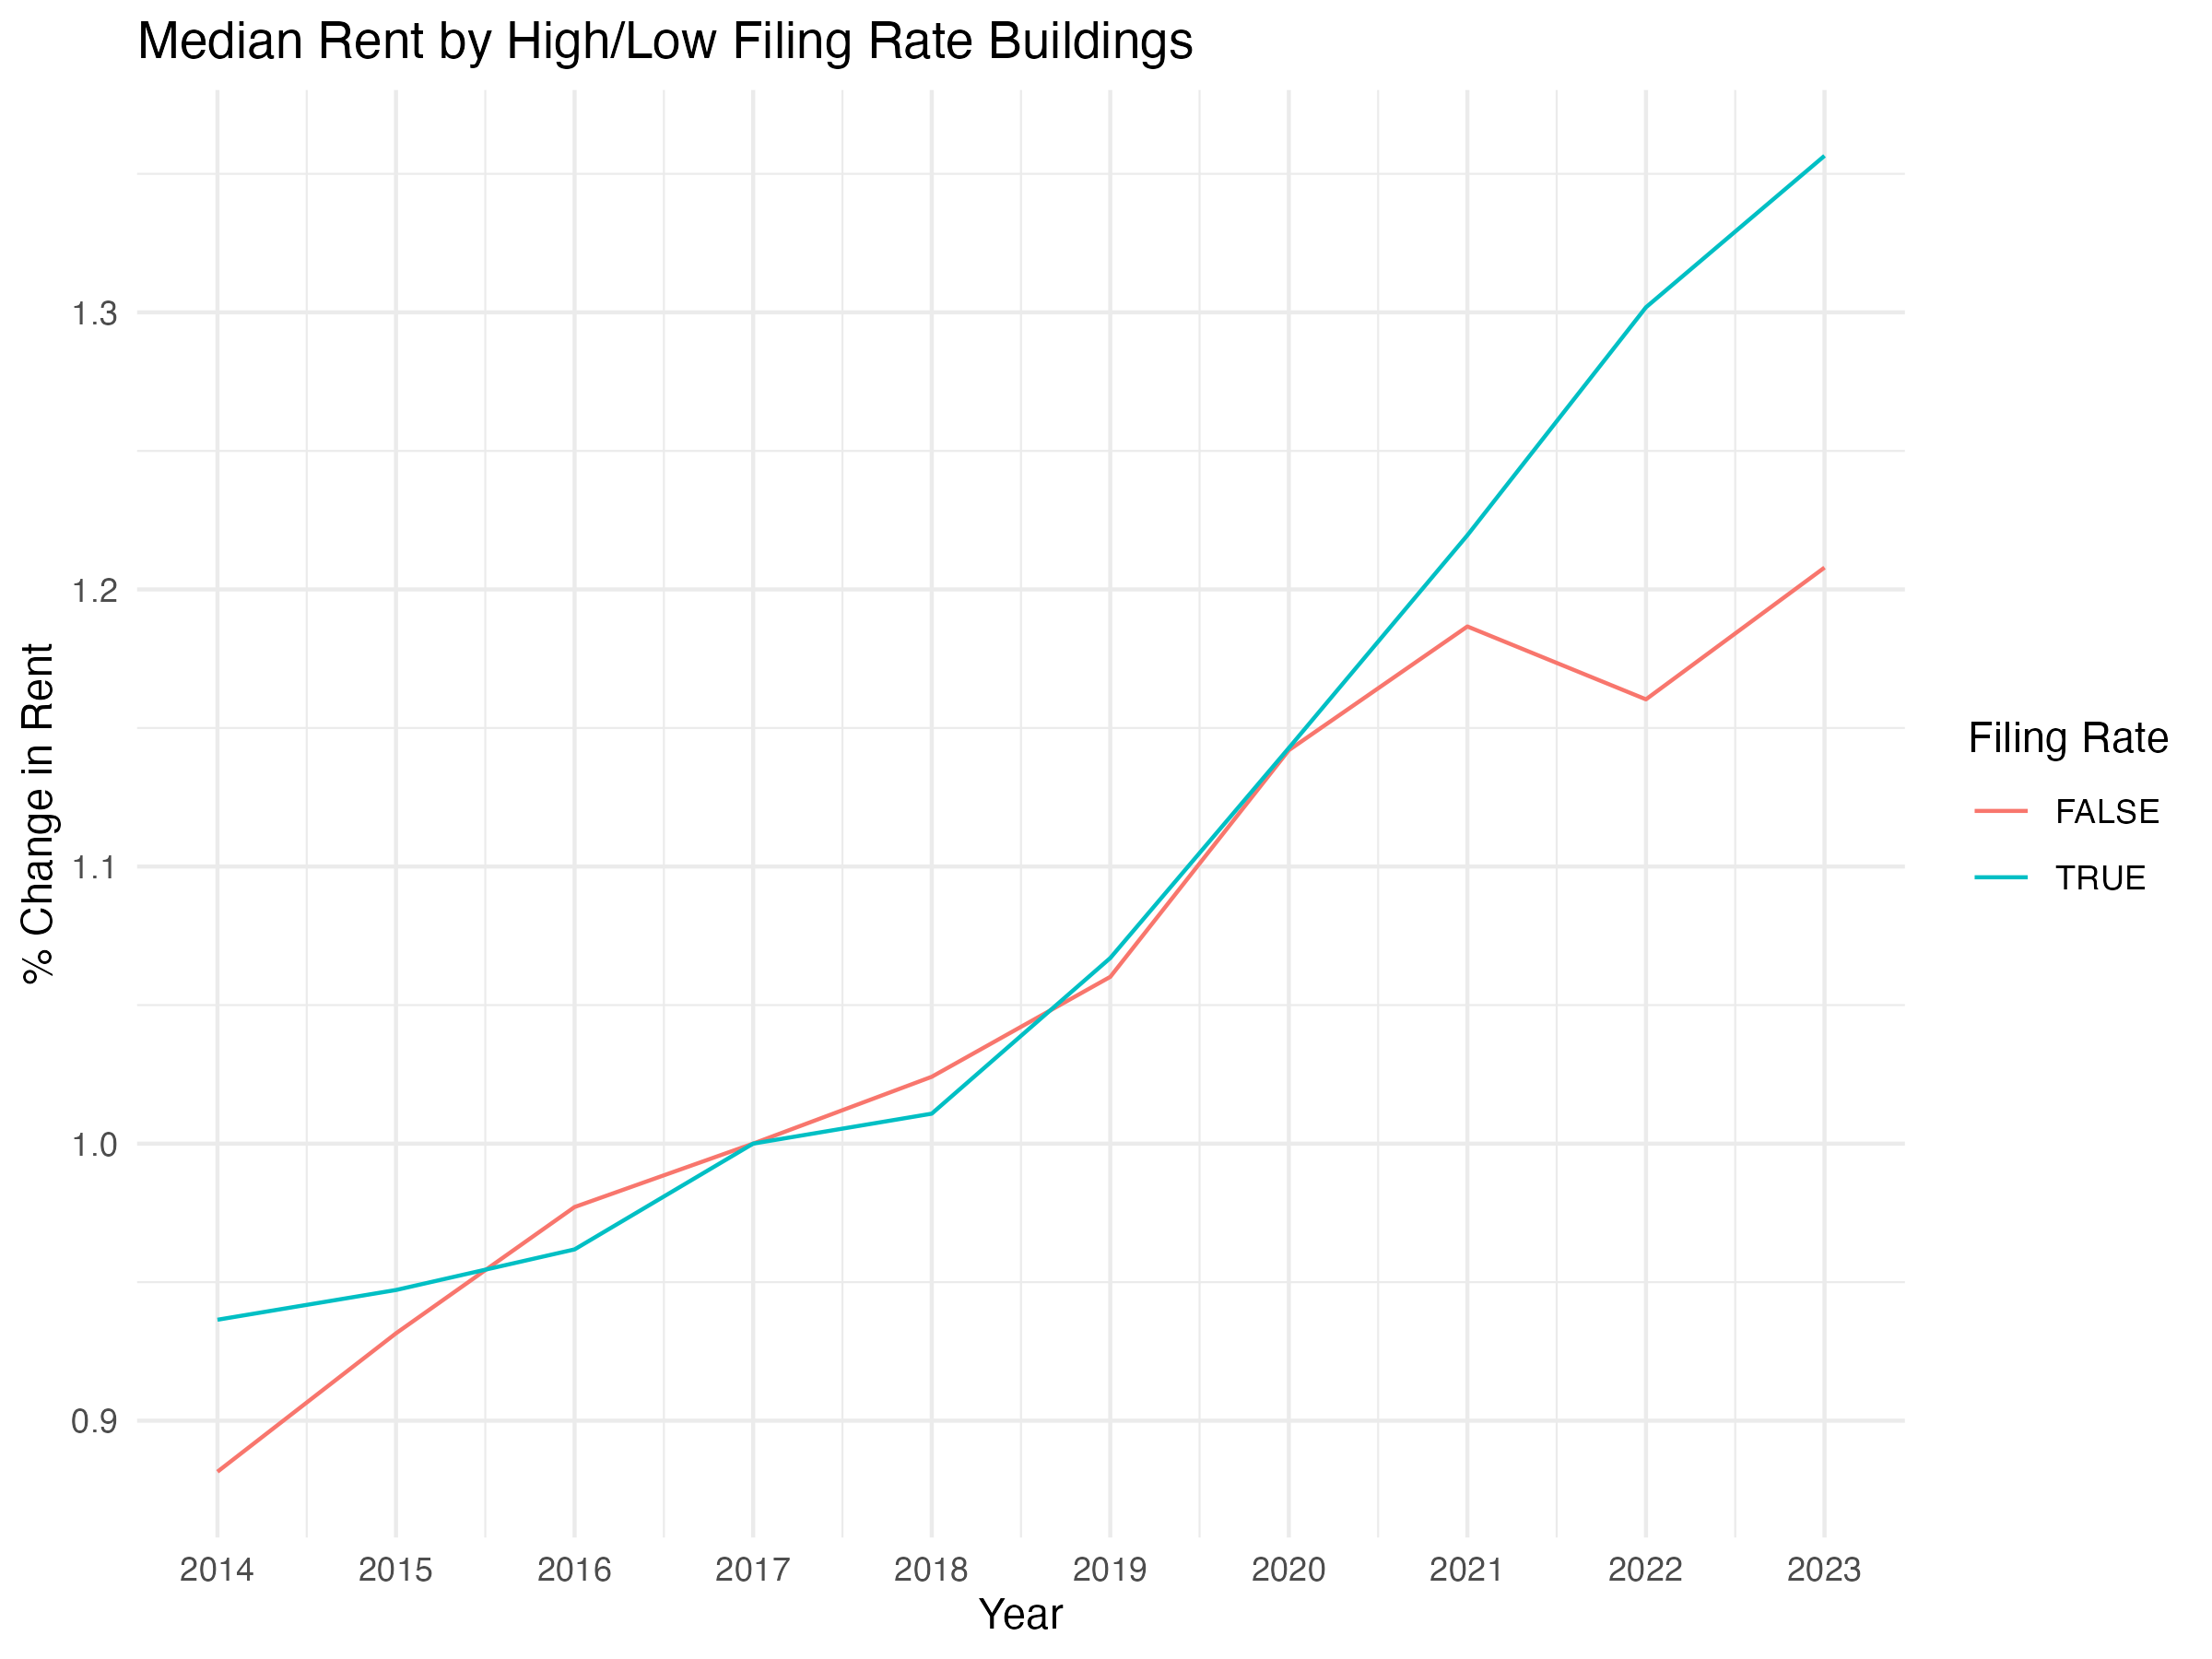
\includegraphics[width=0.5\linewidth]{figs/mean_price_quintile.png}
        \caption{Price Trends By Low Income Units}
        \label{fig:mean-price-quintile}
    \end{figure}
\end{frame}

\begin{frame}{High Evicting Landlords Increased Prices Post-COVID}
    High Evicting Landlords Increased Prices Post-COVID
    \tiny
    \begin{table}[htbp]
   \caption{Price Change Regressions}
   \centering
   \begin{tabular}{lcccc}
      \tabularnewline \midrule \midrule
      Dependent Variable: & \multicolumn{4}{c}{Log Median Rent}\\
                                                   & High Evictors  & High Evictors (within Census Tract) & High Evictors (quintiles) & High Evictors (quintiles within Census Tract) \\   
      Model:                                       & (1)            & (2)                                 & (3)                       & (4)\\  
      \midrule
      \emph{Variables}\\
      High Evictors                                & 0.122$^{***}$  & 0.051$^{***}$                       &                           &   \\   
                                                   & (0.012)        & (0.011)                             &                           &   \\   
      100+ Units                                   & 1.19           & -0.053                              & 0.865                     & -0.035\\   
                                                   & (8,691.3)      & (165.8)                             & (8,707.5)                 & (161.6)\\   
      100+ Units $\times$ Post-COVID Period        & -0.075$^{***}$ & -0.010                              & -0.051$^{**}$             & -0.011\\   
                                                   & (0.026)        & (0.019)                             & (0.024)                   & (0.021)\\   
      2-5 Units $\times$ Post-COVID Period         & -0.002         & 0.028$^{***}$                       & 0.017$^{*}$               & 0.031$^{***}$\\   
                                                   & (0.009)        & (0.008)                             & (0.009)                   & (0.008)\\   
      51-100 Units $\times$ Post-COVID Period      & -0.046         & -0.032$^{*}$                        & -0.031                    & -0.033$^{**}$\\   
                                                   & (0.028)        & (0.016)                             & (0.028)                   & (0.017)\\   
      6-50 Units $\times$ Post-COVID Period        & -0.030$^{*}$   & 0.001                               & -0.006                    & 0.003\\   
                                                   & (0.015)        & (0.012)                             & (0.017)                   & (0.013)\\   
      Post-COVID Period $\times$ corp\_ownerTRUE   & 0.002          & 0.012                               & 0.007                     & 0.013\\   
                                                   & (0.017)        & (0.011)                             & (0.016)                   & (0.011)\\   
      2-5 Units                                    &                & -0.052                              &                           & -0.123\\   
                                                   &                & (245.9)                             &                           & (228.2)\\   
      corp\_ownerTRUE                              &                & 2.13                                &                           & 2.35\\   
                                                   &                & (722.5)                             &                           & (673.6)\\   
      Filing Rate Quintile $=$ 2                   &                &                                     & 0.007                     & 0.011\\   
                                                   &                &                                     & (0.020)                   & (0.019)\\   
      Filing Rate Quintile $=$ 3                   &                &                                     & 0.105$^{***}$             & 0.046$^{**}$\\   
                                                   &                &                                     & (0.022)                   & (0.020)\\   
      Filing Rate Quintile $=$ 4                   &                &                                     & 0.144$^{***}$             & 0.082$^{***}$\\   
                                                   &                &                                     & (0.019)                   & (0.021)\\   
      Filing Rate Quintile $=$ 5                   &                &                                     & 0.168$^{***}$             & 0.088$^{***}$\\   
                                                   &                &                                     & (0.018)                   & (0.019)\\   
      \midrule
      \emph{Fixed-effects}\\
      parcel                                       & Yes            & Yes                                 & Yes                       & Yes\\  
      year                                         & Yes            &                                     & Yes                       & \\  
      Census Tract-year                            &                & Yes                                 &                           & Yes\\  
      \midrule
      \emph{Fit statistics}\\
      Observations                                 & 51,901         & 51,901                              & 51,901                    & 51,901\\  
      \midrule \midrule
      \multicolumn{5}{l}{\emph{Clustered (parcel) standard-errors in parentheses}}\\
      \multicolumn{5}{l}{\emph{Signif. Codes: ***: 0.01, **: 0.05, *: 0.1}}\\
   \end{tabular}
\end{table}

    
\end{frame}


\begin{frame}{New Ideas}
    High Evicting Landlords Left Market Post-COVID
    \tiny
    \begin{table}[]
        \centering
        \begin{tabular}{c|c}
             &  \\
             & 
        \end{tabular}
        \setlength{\LTpost}{0mm}
\begin{longtable}{rrrrrrr}
\caption*{
{\large Philadelphia Rental Housing Stock} \\ 
{\small 2015-2024}
} \\ 
\toprule
Year & Total Units & Units in High Evictor Buildings & Total Rentals & Rentals in High Evictor Buildings & Change in Total Units Since 2019 & Change in High Evictor Units Since 2019 \\ 
\midrule\addlinespace[2.5pt]
2015 & $276,136$ & $11,639$ & $89,949$ & $4,167$ & $-1.9\%$ & $9.6\%$ \\ 
2016 & $267,097$ & $11,971$ & $92,007$ & $3,998$ & $-5.1\%$ & $12.7\%$ \\ 
2017 & $270,982$ & $11,696$ & $94,829$ & $3,968$ & $-3.7\%$ & $10.1\%$ \\ 
2018 & $276,111$ & $11,673$ & $97,019$ & $3,487$ & $-1.9\%$ & $9.9\%$ \\ 
2019 & $281,478$ & $10,623$ & $99,674$ & $3,332$ & $0.0\%$ & $0.0\%$ \\ 
2020 & $277,977$ & $10,488$ & $97,361$ & $3,247$ & $-1.2\%$ & $-1.3\%$ \\ 
2021 & $274,699$ & $10,457$ & $94,540$ & $3,122$ & $-2.4\%$ & $-1.6\%$ \\ 
2022 & $275,988$ & $10,348$ & $92,509$ & $2,971$ & $-2.0\%$ & $-2.6\%$ \\ 
2023 & $282,323$ & $9,966$ & $93,099$ & $2,795$ & $0.3\%$ & $-6.2\%$ \\ 
2024 & $261,337$ & $9,618$ & $83,590$ & $2,607$ & $-7.2\%$ & $-9.5\%$ \\ 
\bottomrule
\end{longtable}
\begin{minipage}{\linewidth}
Data from Philadelphia Housing Rental Registry and Eviction Lab\\
\end{minipage}


        %\caption{Caption}
        \label{tab:placeholder}
    \end{table}
    
\end{frame}



\end{document}
